\chapter{Revisão Bibliográfica}
Neste capitulo serão abordados alguns conceitos e técnicas necessárias para
gerar o mapa de altura proceduralmente, além de apresentar alguns trabalhos
relacionados.

\section{Biomas} %Preciso de mais fontes nesta seção, urgente
Existem mais que um conceito de bioma, um bastante adotado considera bioma como
uma área do espaço geográfico, representada por um tipo uniforme de ambiente, o
mesmo pode ser classificado de acordo com o macroclima, fitofisionomia (formação),
solo e a altitude, os elementos que maus caracterizam os ambientes continentais, 
este é o conceito de \cite{coutinho2006conceito}, usando como base descrições
de \cite{walter1986vegetaccao}.

Porém neste trabalho o conceito de bioma vai ser outro, o resultado deste
vai ser unicamente mapas de altura, então a única característica que é relevante
são as altitudes do solo e seus padrões, descartando dados como tipo da
vegetação e sua distribuição, umidade e entre outros. Então no restante 
do trabalho, quando for usado os termos "característica do bioma", o mesmo vai
se referir a alguma característica de altitude do bioma.

Para fins de restringir o escopo do projeto vamos agrupar os biomas por padrões
de relevo e não por fauna e flora como feito no conceito apresentado acima,
estes biomas serão: cordilheiras (cadeias de montanha), planícies.

\section{Representação das Regiões}
Neste trabalho serão implementadas três maneiras de representar a malha de
regiões, malha de quadrados, malha triangular e diagrma de Voronoi.

Um bioma vai pertencer a um conjunto de regiões, na imagem \ref{fig:squadStripBiomes}
que usa uma malha de quadrados, onde semi-retas vermelhas são fronteiras entre
biomas.
\begin{figure}[H]
    \centering
    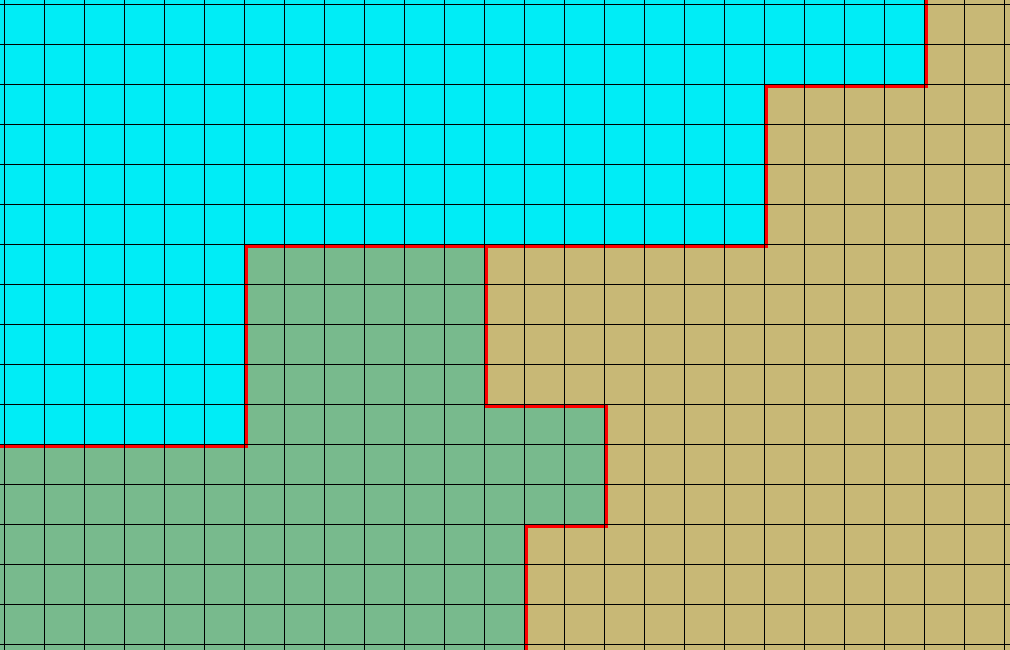
\includegraphics[width=0.7\textwidth]{figuras/squadStripBiomes.png}
    \caption{Malha de quadrados com divisão de biomas}
    \label{fig:squadStripBiomes}
\end{figure}
\subsection{Malhas de quadrado}
Este modelo já apresentado na figura \ref{fig:squadStripBiomes}, nele cada
quadrado é uma região, os vértices armazenados se encontram nos quatro cantos
do quadrado, então um vértice é comum a quatro quadrados, cada um deles
compartilhando o vértice com os quadrados adjacentes, as arestas entre vértices
vizinhos são uma fronteira entre regiões, e tem a possibilidade desta aresta ser
também uma fronteira entre biomas.

Devido ao padrão podemos perceber que não temos a necessidadede armazenar arestas
em memória, já que a mesma só vai existir entre vértices vizinhos, o vértice
$v_{i j}$ tem como vizinhos o conjunto $\{v_{i+1 j}, v_{i-1 j}, v_{i j+1}, v_{i j-1}\}$.
\subsection{Malha triangular}
Usando a mesma base de vértice da malha de quadrados, agora temos uma aresta
adicional, uma diagonal em cada quadrado do modelo anterior, dividindo a região
em duas, cada traingulo sendo uma região, como podemos ver na figura \ref{fig:vbo}.
Agora além do conjunto de arestas do modelo anterior, o vértice $v_{i j}$ tamém tem
aresta para os vértices $\{v_{i+1 j+1}, v_{i-1 j-1}\}$
\begin{figure}[H]
    \centering
    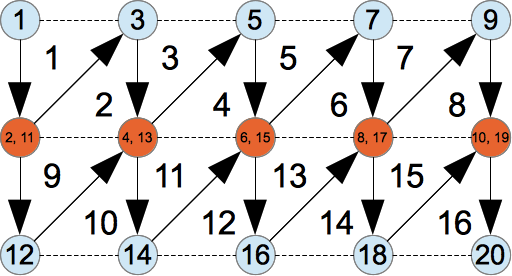
\includegraphics[width=0.5\textwidth]{figuras/vbo.png}
    \caption{Malhas de triângulos, retirado de \cite{androidtrianglestrip}}
    \label{fig:vbo}
\end{figure}


\subsection{Diagrama de Voronoi}
Um diagrama de Voronoi é uma partição no plano para separar regiões, recebendo
como entrada um conjunto de pontos chamados de \textit{sites}, o algoritmo
separa as regiões de cada \textit{site} deixando a fronteira equidistante entre eles
\cite{fortune1987sweepline}.

Como está implementação vai ser não assistida estes sites precisam ser colocados
aleatoriamente e proceduralmente, para não ocorrer aglomerações de site, já
que existe a possibilidade de acontecer na geração de \textit{sites} aleatórios,
será usado o algoritmo de Lloyd's para relaxar os sites, o conjunto dessas
técnicas já foi usado por \cite{patel2010polygonal}, para gerar malha de regiões,
segue uma imagem de seu diagrama na figura \ref{fig:voronoi-2-lloyd}, este diagrama
foi usado para alcançar o resultado já mostrado na ilustração \ref{fig:voronoi-map-goal-distorted}.
\begin{figure}[H]
    \centering
    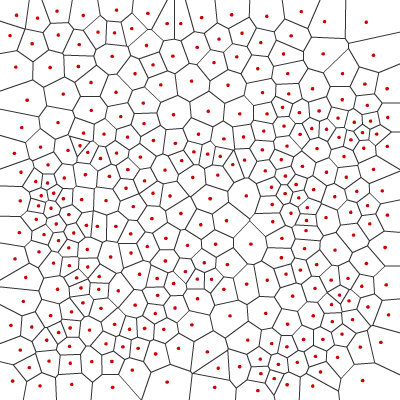
\includegraphics[width=0.5\textwidth]{figuras/voronoi-2-lloyd.png}
    \caption{Diagrama de Voronoi com algoritmo de Lloyd's aplicado, por \cite{patel2010polygonal}}
    \label{fig:voronoi-2-lloyd}
\end{figure}

\section{Ruído de Perlin}

\section{Mapas de Altura}

\section{Trabalhos Relacionados}

%correção: preciso colocar trabalhos fora deste vínculo e quem sabe adicionar uma seção
%sobre
%Ainda não sei ao certo quais são os trabalhos relacionados que vou apresentar
\subsection{Trabalho de Carli}

